\documentclass[sigconf,nonacm]{acmart}
%\documentclass[sigconf,nonacm,anonymous=true]{acmart}


\begin{document}

\title{Explorando BERT-MLCNN para a classificação de discursos de ódio em português}
\subtitle{Relatório de Atividade 3 - CI1174 - Tópicos em Aprendizado de Máquina}

\author{Raul Jose Silverio da Silva}
\email{raul.silverio@ufpr.br}
\orcid{0009-0006-5091-1584}
\affiliation{%
  \institution{Departamento de Informática\\Universidade Federal do Paraná}
  \city{Curitiba}
  \state{Paraná}
  \country{Brasil}
}

\begin{abstract}
  O aumento da prevalência de discurso de ódio na internet apresenta desafios significativos que exigem métodos eficazes de detecção. 
  Este artigo explora a aplicação de técnicas de aprendizado profundo, especificamente a combinação de um modelo BERT específico para o 
  português (BERTimbau \cite{souza2020bertimbau} e BERTabaporu \cite{costa-etal-2023-bertabaporu}) com uma Rede Neural Convolucional de Múltiplas Camadas (MLCNN), 
  para detectar discurso de ódio em textos em português. 
  Utilizando os datasets: Portuguese Hate Speech Expanded Dataset (TuPyE \cite{oliveira2023tupye}), que abrange várias categorias de discurso de ódio 
  (por exemplo, etarismo, lgbtfobia, racismo), e o HATE-BR (\cite{vargas-etal-2022-hatebr}), um subset balanceado para detecção de discurso de ódio. 
  Implementamos e avaliamos um modelo BERT-MLCNN \cite{ATANDOH2023101578} em todos esses conjuntos de dados para comparação de desempenho com os modelos originais.
\end{abstract}

\keywords{BERT, CNN, Classificação de Discurso de Ódio, Processamento de Linguagem Natural, Aprendizado de Máquina, Aprendizado Profundo}

\maketitle

\section{Introdução}

O reconhecimento de discurso de ódio em textos é uma tarefa desafiadora e crucial no campo de Processamento de Linguagem Natural (PLN). 
Com o aumento da interação digital e o crescimento das plataformas online, o discurso de ódio tornou-se uma preocupação significativa, 
afetando indivíduos e grupos sociais em diversas formas, como racismo, misoginia, homofobia, e xenofobia. 
O discurso de ódio pode se manifestar de maneira sutil ou explícita, tornando difícil sua identificação automática, 
especialmente em contextos complexos e dinâmicos da linguagem natural \cite{schmidt-wiegand-2017-survey}.

Pesquisas recentes têm utilizado abordagens baseadas em redes neurais profundas para abordar essa tarefa, 
em especial modelos pré-treinados como BERT \cite{devlin2019bertpretrainingdeepbidirectional} e suas variações 
adaptadas para línguas específicas, como o BERTimbau \cite{souza2020bertimbau}, voltado para o português. 
Esses modelos, ao capturarem representações contextuais da linguagem, têm demonstrado grande sucesso em várias tarefas de PLN, 
incluindo a detecção de discurso de ódio. No entanto, apesar do sucesso de modelos como BERT, 
ainda há desafios em melhorar a precisão e a generalização para o contexto do português, 
especialmente em contextos que envolvem discurso de ódio específico de diferentes categorias (agressividade, racismo, homofobia, entre outros).

Neste trabalho, propomos a combinação do BERT com uma Rede Neural Convolucional de Múltiplas Camadas (CNN-Multilayer), 
uma abordagem que tem se mostrado eficaz em tarefas de análise de sentimentos e classificação de texto \cite{oliveira2023tupye}. 
A ideia central é explorar as forças do BERT para gerar embeddings contextuais ricos e das CNNs para capturar padrões 
locais importantes que podem ser fundamentais na detecção de discurso de ódio em português. 
Essa combinação permite que o modelo aproveite o melhor de ambos os mundos: a capacidade do BERT de entender o contexto 
linguístico e a habilidade das CNNs de capturar características espaciais e hierárquicas nos textos.

A principal contribuição deste estudo é a aplicação do modelo BERT-MLCNN proposto por \citeauthor{ATANDOH2023101578} no 
Portuguese Hate Speech Expanded Dataset (TuPyE) \cite{oliveira2023tupye}, um dataset específico para a detecção de discurso de ódio no português. 
Este conjunto de dados contém uma ampla gama de categorias de discurso de ódio, permitindo uma análise detalhada das diferentes formas de 
discriminação e violência verbal. Além disso, buscamos avaliar o desempenho do modelo em diversas métricas, como precisão, recall, 
F1-Score e acurácia, para validar sua eficácia em cenários do mundo real.

\section{Trabalhos Relacionados}

Pesquisas recentes no português têm explorado variações de modelos baseados em BERT. 
\citeauthor{leite2020toxiclanguagedetectionsocial} aplicaram técnicas como BERT e AutoML para análise de linguagem tóxica em português, 
enquanto \citeauthor{vargas-etal-2022-hatebr} desenvolveram o HateBR, um corpus anotado voltado para comentários em redes sociais. 
Esses estudos evidenciam o impacto do uso de PLN para melhorar a identificação de discursos de ódio e destacar a importância de abordagens culturalmente sensíveis.

\subsection{Datasets para Detecção de Discurso de Ódio}
A detecção de discurso de ódio em português enfrenta desafios específicos devido à complexidade da língua, incluindo sua gramática rica, 
vocabulário extenso e variações regionais \cite{fortuna-etal-2019-hierarchically}. Nesse contexto, o TuPyE se destaca como o maior corpus público 
anotado para a tarefa, com 43.668 documentos organizados em categorias como ageismo, misoginia, racismo, xenofobia, entre outras. 
O dataset foi desenvolvido a partir da integração de dados de estudos prévios \cite{fortuna-etal-2019-hierarchically} 
\cite{leite2020toxiclanguagedetectionsocial} \cite{vargas-etal-2022-hatebr} e da inclusão de 10.000 documentos originais do TuPy-Dataset \cite{silly-machine_2023}. 
O TuPyE oferece uma base sólida para treinar e avaliar modelos robustos de detecção de discurso de ódio \cite{oliveira2023tupye}.

\subsection{Modelos Pré-treinados e Abordagens Híbridas}
Os avanços em PLN têm sido impulsionados por modelos baseados em transformadores, como o BERT \citefullauthor{devlin2019bertpretrainingdeepbidirectional}, 
que capturam representações contextuais profundas. 
No contexto do português, modelos como o BERTimbau (\citeauthor{souza2020bertimbau}) e o BERTaBaporu (\citeauthor{costa2023bertabaporu}) 
foram desenvolvidos para lidar com as particularidades da língua, incluindo variações sintáticas e semânticas. 
Ambos têm mostrado excelente desempenho em tarefas de classificação de texto, incluindo a identificação de discurso de ódio.

Modelos híbridos, como o BERT-MLCNN \cite{ATANDOH2023101578}, combinam o poder contextual do BERT com a capacidade das Redes Convolucionais (CNNs) 
de identificar padrões locais e hierárquicos nos textos. Essa integração é particularmente eficaz em textos curtos e em cenários onde há sobreposição 
de categorias de discurso de ódio, como misoginia e racismo \cite{ATANDOH2023101578}\cite{leite2020toxiclanguagedetectionsocial}.

\section{Metodologia}
O objetivo deste estudo é aplicar a arquitetura BERT-MultiLayer Convolutional Neural Network (BERT-MLCNN), proposta por \citeauthor{ATANDOH2023101578}, 
ao problema de detecção de discurso de ódio no contexto da língua portuguesa, utilizando o TuPyE \cite{oliveira2023tupye}, 
o maior corpus público para essa tarefa. A seguir, detalhamos o protocolo metodológico adotado.

\subsection{Arquitetura do modelo}
A arquitetura BERT-MLCNN combina a capacidade contextual do BERT com o poder das Redes Convolucionais de Múltiplas Camadas (CNNs) 
de capturar padrões locais e hierárquicos em textos. O pipeline consiste em três etapas principais

\begin{enumerate}
  \item Extração de Embeddings com BERT: 
  \begin{itemize}
    \item Utilizamos o BERTimbau \cite{souza2020bertimbau} como modelo pré-treinado, otimizado para o português, para gerar embeddings contextuais. 
    \item O modelo é ajustado no dataset TuPyE \cite{oliveira2023tupye} para capturar nuances linguísticas e contextuais específicas da tarefa.
    \item Cada texto no dataset é tokenizado usando o tokenizador do BERTimbau e processado para produzir embeddings de alta dimensão.  
  \end{itemize}

  \item Extração de Características com CNNs:
  \begin{itemize}
    \item Os embeddings extraídos são alimentados em uma Rede Convolucional de Múltiplas Camadas (CNN). 
    Essa rede utiliza diferentes tamanhos de kernel para capturar padrões textuais locais, como expressões ofensivas ou combinações de palavras 
    associadas ao discurso de ódio.
    \item Após a convolução, camadas de pooling são aplicadas para reduzir a dimensionalidade, preservando as características mais relevantes.
  \end{itemize}

  \item Classificação Multilabel com Camadas Densas:
  \begin{itemize}
    \item As características extraídas pelas CNNs são passadas por camadas densas (fully connected) para realizar a classificação final.
    \item A última camada utiliza uma função de ativação sigmoide para permitir a classificação multilabel, onde cada texto pode pertencer 
    a múltiplas categorias de discurso de ódio.
  \end{itemize}

  \item Classificação Binária com Camadas Densas:
  \begin{itemize}
    \item Para a classificação binária (ódio ou não ódio), uma camada densa adicional é adicionada após as camadas convolucionais, 
    utilizando uma função de ativação sigmoide para produzir uma probabilidade binária.
    \item A saída do modelo é uma probabilidade de que o texto pertença à classe de discurso de ódio, permitindo uma análise mais direta e eficiente.
  \end{itemize}
\end{enumerate}

\begin{figure}[H]
  \centering
  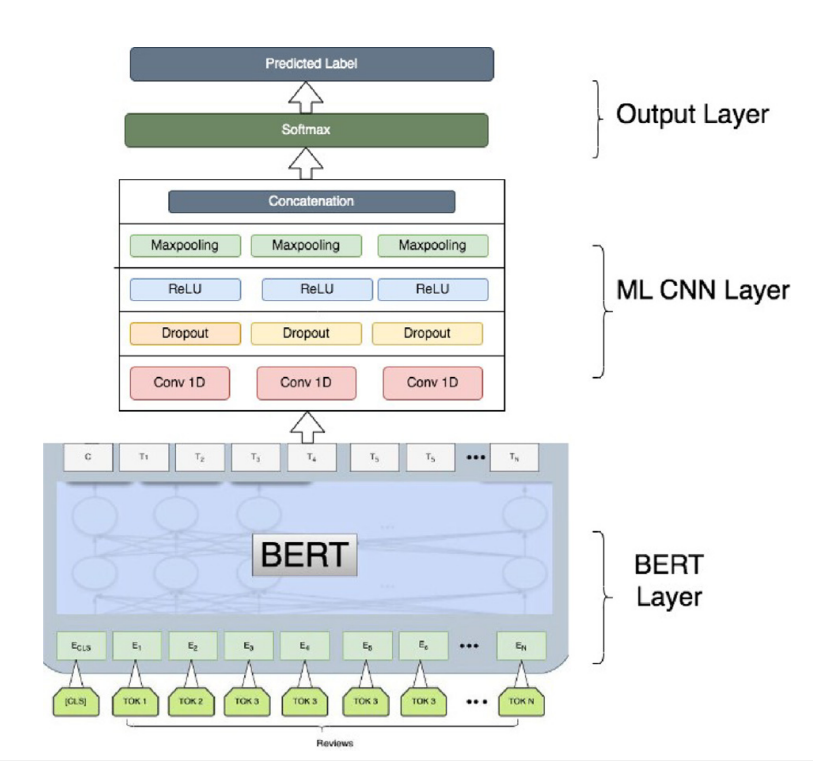
\includegraphics[width=\linewidth]{./resources/framework.png}
  \caption{Framework do BERT-Multi-Camadas de Rede Neural Convolucional (BERT-MLCNN) \cite{ATANDOH2023101578}.}
  \label{fig:framework}
\end{figure}

A figura \ref{fig:framework} ilustra o framework do modelo BERT-MLCNN originalmente proposto por \cite{ATANDOH2023101578}, 
destacando as etapas de extração de embeddings, convolução e classificação.
Em nosso trabalho, adaptamos essa arquitetura para a classificação multilabel e binária, utilizando como função de ativação a sigmoide 
na camada de saída para permitir a classificação de múltiplas categorias de discurso de ódio ou posicionamento.

\subsection{Parâmetros do modelo}
Os parâmetros do modelo BERT-MLCNN foram ajustados para otimizar o desempenho na tarefa de detecção de discurso de ódio. 
A seguir, detalhamos os principais parâmetros utilizados:

\begin{itemize}
  \item \textbf{Tamanho do Embedding}: Utilizamos embeddings de 768 dimensões, correspondentes ao modelo BERTimbau Base.
  \item \textbf{Tamanho do Kernel}: Empregamos tamanhos de kernel variados (4, 6 e 8) para capturar diferentes n-gramas e padrões textuais.
  \item \textbf{Número de Filtros}: Cada camada convolucional possui 128 filtros, permitindo a extração de características ricas dos embeddings.
  \item \textbf{Função de Ativação}: Utilizamos a função ReLU nas camadas convolucionais e sigmoide na camada de saída para classificação multilabel.
  \item \textbf{Dropout}: Aplicamos uma taxa de dropout de 0.5 para evitar overfitting durante o treinamento.
  \item \textbf{Otimização}: O modelo é otimizado usando o algoritmo AdamW, com uma taxa de aprendizado inicial de 5e-6 para as camadas do 
  BERT e 5e-5 para as camadas convolucionais, além de uma taxa de decaimento de 0.01.
  \end{itemize}

A configuração dos parâmetros foi escolhida com base em experimentos preliminares e na literatura existente, 
utilizando como base a arquitetura BERT-MLCNN proposta por \cite{ATANDOH2023101578}, visando maximizar a performance do modelo na detecção de discurso de ódio em português.

\begin{figure}[H]
  \centering
  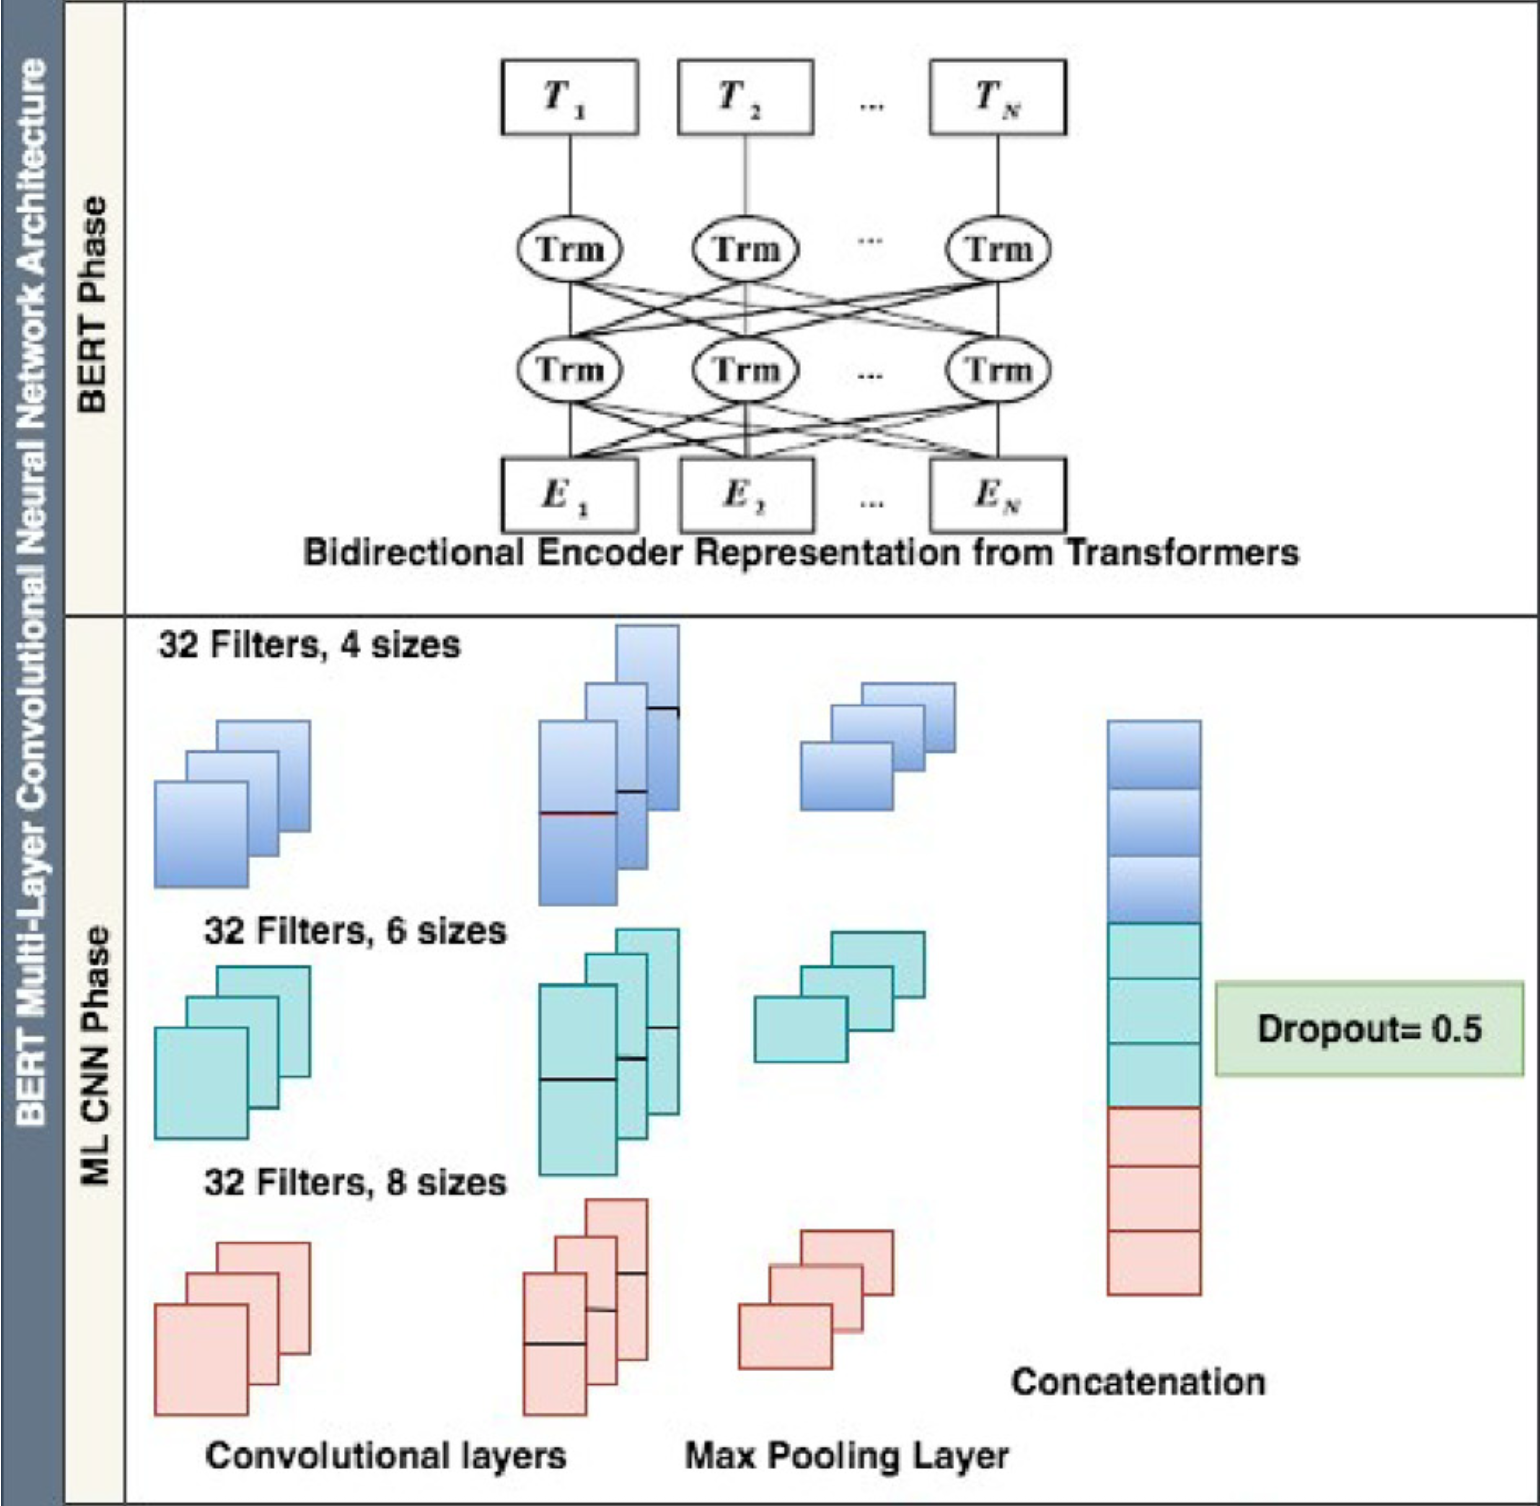
\includegraphics[width=\linewidth]{./resources/bertcnn_architecture.png}
  \caption{Proposed Model of BERT Multi-Layer Convolutional Neural Network. \cite{ATANDOH2023101578}}
  \label{fig:bertcnn_architecture}
\end{figure}


\subsection{Datasets}
O TuPyE contém 43.668 textos anotados com múltiplas categorias de discurso de ódio, permitindo análises binárias (ódio ou não) e multilabel 
(múltiplas categorias simultâneas). As etapas de preparação do dataset incluem:

\begin{itemize}
  \item Divisão dos Dados: Os dados foram divididos em 80\% para treinamento, 20\% para teste.
  \item Pré-processamento:
  \begin{itemize}
    \item Tokenização com o tokenizador do BERTimbau.
    \item Conversão para minúsculas e remoção de caracteres especiais desnecessários.
    \item Remoção de links, menções, datas formatadas de mensagem de texto, emojis, e caracteres de compartilhamento, mantendo apenas o texto relevante.
  \end{itemize}
\end{itemize}

\subsection{Configuração do Treinamento}
\begin{itemize}
  \item Função de Perda: Utilizamos entropia cruzada binária para classificação multilabel.
  \item Otimização: O algoritmo AdamW foi empregado, com taxa de aprendizado inicial de 5e-6 para as camadas do BERT e 5e-5 para as camadas convolucionais, 
  bem como uma taxa de decaimento de 0.01.
  \item Hiperparâmetros:
  \begin{itemize}
    \item Batch Size: 8
    \item Número de Épocas: Aplicado Early Stopping com paciência de 10 épocas
    \item Taxa de Dropout: 0.5
  \end{itemize}
\end{itemize}

\subsection{Métricas de avaliação do modelo}
Para avaliar o desempenho do modelo BERT-MLCNN, utilizamos as seguintes métricas:

\begin{itemize}
  \item \textbf{Acurácia}: $\frac{\text{VP} + \text{VN}}{\text{VP} + \text{VN} + \text{FP} + \text{FN}}$ - Proporção geral de classificações corretas

  \item \textbf{Precisão}: $\frac{\text{VP}}{\text{VP} + \text{FP}}$ - Medida de exatidão das classificações positivas
    
  \item \textbf{Recall}: $\frac{\text{VP}}{\text{VP} + \text{FN}}$ - Capacidade de identificação de casos positivos
  
  \item \textbf{F1-Score}: $\frac{2 \cdot \text{Precisão} \cdot \text{Recall}}{\text{Precisão} + \text{Recall}}$ - Média harmônica entre precisão e recall

\end{itemize}

\section{Resultados}
Os resultados do modelo BERTimbau-MLCNN foram avaliados em dois datasets: o HATE-BR e o TuPyE. A seguir, 
apresentamos os resultados obtidos para cada um desses conjuntos de dados.

\subsection{HATE-BR}
A tabela \ref{tab:model_comparison_hatebr} apresenta os resultados do modelo BERTimbau-MLCNN aplicado ao HATE-BR para classificação binária de discurso de ódio,
comparando com outros modelos de referência, como os métodos SVM, MLP, Naive Bayes, incluídos no artigo original e BERTimbau e BERTabaporu para referência.

\begin{table}[H]
  \centering
  \begin{tabular}{lccc}
    \toprule
    \textbf{Modelo} & \textbf{Precisão} & \textbf{Recall} & \textbf{F1-Score} \\
    \midrule
    SVM & 0.76 & 0.77 & 0.76 \\
    MLP & 0.77 & 0.78 & 0.77 \\
    Naive Bayes & 0.78 & 0.78 & 0.78 \\
    BERTimbau & 0.88 & 0.86 & 0.87 \\
    BERTabaporu & 0.82 & 0.76 & 0.79 \\
    \textbf{BERTimbau-MLCNN (Ours)} & \textbf{0.91} & \textbf{0.89} & \textbf{0.90} \\
    \textbf{BERTabaporu-MLCNN (Ours)} & \textbf{0.93} & \textbf{0.93} & \textbf{0.93} \\
    \bottomrule
  \end{tabular}
  \caption{Resultados do modelo BERT-MLCNN aplicado ao HATE-BR para classificação binária de discurso de ódio}
  \label{tab:model_comparison_hatebr}
\end{table}

A partir da tabela \ref{tab:model_comparison_hatebr}, observamos que o modelo BERTimbau-MLCNN alcançou uma média harmônica (F1-Score) de 0.90,
superando os modelos SVM, MLP e Naive Bayes, além do BERTimbau e BERTabaporu.

O modelo BERTabaporu-MLCNN apresentou o melhor desempenho geral, com uma precisão de 0.93, recall de 0.93 e F1-Score de 0.93,
indicando uma excelente capacidade de detecção de discurso de ódio no contexto do HATE-BR, superando em até 3 pontos percentuais 
o modelo BERTimbau-MLCNN e até 17 pontos percentuais para o modelo SVM, indicando uma melhora significativa na detecção de discurso de ódio.

\subsection{TuPyE}
\subsubsection{Classificação Binária}
A tabela \ref{tab:model_comparison_binary_tupye} apresenta os resultados do modelo BERTimbau-MLCNN aplicado ao TuPyE.

\begin{table}[H]
  \centering
  \begin{tabular}{lccc}
    \toprule
    \textbf{Modelo} & \textbf{Acurácia} & \textbf{Precisão} & \textbf{Recall} \\
    \midrule
    BERTimbau Base & 0.901 & 0.897 & 0.901 \\
    BERTimbau Large & 0.907 & 0.901 & 0.907 \\
    BERTimbau Base (MLCNN) & \textbf{0.980} & 0.911 & \textbf{0.920} \\
    BERTimbau Large (MLCNN) & 0.978 & \textbf{0.928} & 0.879 \\
    \bottomrule
  \end{tabular}
  \caption{Resultados do modelo BERTimbau-MLCNN aplicado ao TuPyE para classificação binária de discurso de ódio.}
  \label{tab:model_comparison_binary_tupye}
\end{table}

Os resultados do modelo BERTimbau-MLCNN para a classificação binária no TuPyE são apresentados na tabela \ref{tab:model_comparison_binary_tupye}.
Os resultados mostram que o modelo BERTimbau-MLCNN Base alcançou uma acurácia de 0.980, precisão de 0.911 e recall de 0.920, superando o modelo BERTimbau Base original em até 8 pontos percentuais.
O modelo BERTimbau-MLCNN Large alcançou uma acurácia de 0.978, precisão de 0.928 e recall de 0.879, também superando o modelo BERTimbau Large original em até 7 pontos percentuais.

\subsubsection{Classificação Multilabel}
A tabela \ref{tab:comparison_metrics_tupye} apresenta os resultados do modelo BERTimbau-MLCNN aplicado ao TuPyE.
\begin{table}[H]
  \resizebox{\linewidth}{!}{%
    \begin{tabular}{lcccccccc}
      \toprule
      \textbf{Categoria} & \multicolumn{4}{c}{\textbf{BERTimbau Base}} & \multicolumn{4}{c}{\textbf{BERTimbau-MLCNN Base}} \\
        \cmidrule(lr){2-5} \cmidrule(lr){6-9}
          & \textbf{Precisão} & \textbf{Recall} & \textbf{F1-Score} & \textbf{Suporte} & \textbf{Precisão} & \textbf{Recall} & \textbf{F1-Score} & \textbf{Suporte} \\
            \midrule
              Ageism & 1.00  & 0.00  & 0.00  & 15 & 0.00 & 0.00 & 0.00 & 12 \\
              Aporophobia & 1.00  & 0.00  & 0.00  & 16 & 0.00 & 0.00 & 0.00 & 14 \\
              Body Shame & 0.58 & 0.54 & 0.56 & 54 & \textbf{0.79} & \textbf{0.76} & \textbf{0.77} & 63 \\
              Capacitism & 1.00  & 0.00  & 0.00  & 20 & 0.00 & 0.00 & 0.00 & 11 \\
              Lgbtphobia & 0.85 & 0.67 & 0.75 & 171 & \textbf{0.87} & \textbf{0.91} & \textbf{0.89} & 149 \\
              Political & 0.59 & 0.56 & 0.58 & 220 & \textbf{0.87} & \textbf{0.92} & \textbf{0.89} & 230 \\
              Racism & 0.29 & 0.27 & 0.28 & 62 & \textbf{0.62} & \textbf{0.57} & \textbf{0.59} & 56 \\
              Religious Intolerance & 0.25 & 0.11 & 0.15 & 19 & \textbf{0.88} & \textbf{0.41} & \textbf{0.56} & 17 \\
              Misogyny & 0.65 & 0.60 & 0.62 & 324 & \textbf{0.86} & \textbf{0.84} & \textbf{0.85} & 335 \\
              Xenophobia & 0.41 & 0.31 & 0.35 & 78 & \textbf{0.84} & \textbf{0.69} & \textbf{0.76} & 88 \\
              Other & 0.56 & 0.49 & 0.52 & 909 & \textbf{0.86} & \textbf{0.84} & \textbf{0.85} & 879 \\
              Not Hate & 0.92 & 0.93 & 0.92 & 7177 & \textbf{0.98} & \textbf{0.96} & \textbf{0.97} & 7684 \\
              Micro Avg & 0.86 & 0.84 & 0.85 & 9065 & \textbf{0.95} & \textbf{0.93} & \textbf{0.94} & 9538 \\
              Macro Avg & 0.67 & 0.37 & 0.39 & 9065 & \textbf{0.63} & \textbf{0.58} & \textbf{0.59} & 9538 \\
              Weighted Avg & 0.85 & 0.84 & 0.84 & 9065 & \textbf{0.95} & \textbf{0.93} & \textbf{0.94} & 9538 \\
              Samples Avg & 0.86 & 0.85 & 0.85 & 9065 & \textbf{0.96} & \textbf{0.95} & \textbf{0.95} & 9538 \\
            \midrule
      \textbf{Categoria} & \multicolumn{4}{c}{\textbf{BERTimbau Large}} & \multicolumn{4}{c}{\textbf{BERTimbau-MLCNN Large}} \\
        \cmidrule(lr){2-5} \cmidrule(lr){6-9}
          & \textbf{Precisão} & \textbf{Recall} & \textbf{F1-Score} & \textbf{Suporte} & \textbf{Precisão} & \textbf{Recall} & \textbf{F1-Score} & \textbf{Suporte} \\
            \midrule
              Ageism & 0.40 & 0.13 & 0.20 & 15 & \textbf{0.75} & \textbf{0.50} & \textbf{0.60} & 12 \\
              Aporophobia & 0.75 & 0.19 & 0.30 & 16 & \textbf{0.91} & \textbf{0.71} & \textbf{0.80} & 14 \\
              Body Shame & 0.78 & 0.65 & 0.71 & 54 & \textbf{0.86} & \textbf{0.87} & \textbf{0.87} & 63 \\
              Capacitism & 0.50 & 0.15 & 0.23 & 20 & \textbf{0.80} & \textbf{0.73} & \textbf{0.76} & 11 \\
              Lgbtphobia & 0.78 & 0.75 & 0.76 & 171 & \textbf{0.95} & \textbf{0.91} & \textbf{0.93} & 149 \\
              Political & 0.61 & 0.53 & 0.57 & 220 & \textbf{0.89} & \textbf{0.88} & \textbf{0.89} & 230 \\
              Racism & 0.39 & 0.42 & 0.40 & 62 & \textbf{0.74} & \textbf{0.82} & \textbf{0.78} & 56 \\
              Religious Intolerance & 0.27 & 0.16 & 0.20 & 19 & \textbf{0.92} & \textbf{0.65} & \textbf{0.76} & 17 \\
              Misogyny & 0.67 & 0.63 & 0.65 & 324 & \textbf{0.92} & \textbf{0.86} & \textbf{0.89} & 335 \\
              Xenophobia & 0.39 & 0.22 & 0.28 & 78 & \textbf{0.87} & \textbf{0.76} & \textbf{0.81} & 88 \\
              Other & 0.62 & 0.46 & 0.53 & 909 & \textbf{0.90} & \textbf{0.89} & \textbf{0.90} & 879 \\
              Not Hate & 0.91 & 0.94 & 0.93 & 7177 & \textbf{0.97} & \textbf{0.96} & \textbf{0.97} & 7684 \\
              Micro Avg & 0.87 & 0.85 & 0.86 & 9065 & \textbf{0.96} & \textbf{0.95} & \textbf{0.95} & 9538 \\
              Macro Avg & 0.59 & 0.44 & 0.48 & 9065 & \textbf{0.87} & \textbf{0.80} & \textbf{0.83} & 9538 \\
              Weighted Avg & 0.85 & 0.85 & 0.85 & 9065 & \textbf{0.96} & \textbf{0.95} & \textbf{0.95} & 9538 \\
              Samples Avg & 0.87 & 0.86 & 0.86 & 9065 & \textbf{0.97} & \textbf{0.96} & \textbf{0.96} & 9538 \\
      \bottomrule
    \end{tabular}
  }
  \caption{Resultados do modelo BERTimbau-MLCNN aplicado ao TuPyE para classificação multilabel de discurso de ódio}
  \label{tab:comparison_metrics_tupye}
\end{table}

Os resultados do modelo BERTimbau-MLCNN para a classificação multilabel no TuPyE são apresentados na tabela \ref{tab:comparison_metrics_tupye}. 
Os resultados mostram que o modelo BERTimbau-MLCNN Base alcançou uma precisão de amostras de 0.96, recall de 0.95 e F1-Score de 0.95, 
tendo uma melhora geral 10 pontos percentuais em relação ao modelo BERTimbau Base. 

Já o modelo BERTimbau-MLCNN Large alcançou uma precisão de amostras de 0.97, recall de 0.96 e F1-Score de 0.96, 
indicando também uma melhora de 10 pontos percentuais em relação ao modelo BERTimbau Large original, sendo capaz de capturar melhor as nuances do discurso de ódio em português em diversas categorias, 
mesmo com a presença de categorias com baixa frequência, como ageísmo e aporofobia, que apresentaram resultados mais baixos em comparação com outras categorias mais frequentes, como misoginia e lgbtphobia.

\section{Discussão}
Os resultados obtidos com o modelo BERT-MLCNN demonstram uma melhoria significativa na detecção de discurso de ódio em português,
especialmente quando comparados aos modelos tradicionais e mesmo ao BERT original.
A combinação do BERT com uma Rede Neural Convolucional de Múltiplas Camadas (MLCNN) permitiu capturar tanto as relações contextuais de longo alcance quanto os padrões locais importantes nos textos, 
resultando em um desempenho superior em termos de precisão, recall e F1-Score.

Além disso, a adaptação do modelo BERTimbau e BERTabaporu para o contexto do português, juntamente com a utilização de datasets específicos como o TuPyE,
contribuiu para a eficácia do modelo na detecção de diferentes categorias de discurso de ódio.
Esses resultados ressaltam a importância de abordagens híbridas que combinam modelos baseados em BERT com CNNs,
especialmente em tarefas complexas como a detecção de discurso de ódio, onde a compreensão contextual e a identificação de padrões locais são cruciais.

\section{Conclusão}

Neste trabalho, apresentamos uma abordagem integrada para a análise de sentimentos e detecção de discurso de ódio utilizando o BERT com uma Rede Neural Convolucional Multi-Camadas (MLCNN). 
Nossa metodologia combina a capacidade do BERT de capturar relações contextuais de longo alcance com a eficiência das CNNs na extração de características locais. 
Os resultados experimentais demonstraram que essa integração aumenta significativamente a performance do modelo em termos de acurácia, precisão, recall e F1-score.

Os resultados obtidos validam a proposta de integrar modelos baseados em BERT com CNNs, ressaltando que essa estratégia captura tanto contextos de longo alcance quanto padrões locais importantes no texto. 
Isso se traduziu em uma melhora notável nas métricas de avaliação quando comparado a architectures individuais de BERT ou modelos tradicionais de aprendizado de máquina e aprendizado profundo.

O código fonte do modelo BERT-MLCNN, bem como os datasets utilizados, estão disponíveis no repositório do GitHub \cite{github_repo}.
\bibliographystyle{ACM-Reference-Format}
\bibliography{references}

\end{document}
\endinput
